\documentclass[crop,tikz]{standalone}
\usepackage{tkz-euclide}
\usetikzlibrary{arrows.meta}
\usetkzobj{all}
\usetikzlibrary{shapes}


\tikzstyle{myarrows}=[line width=1mm,draw=blue,-triangle 45,postaction={draw, line width=3mm, shorten >=4mm, -}]
\begin{document}

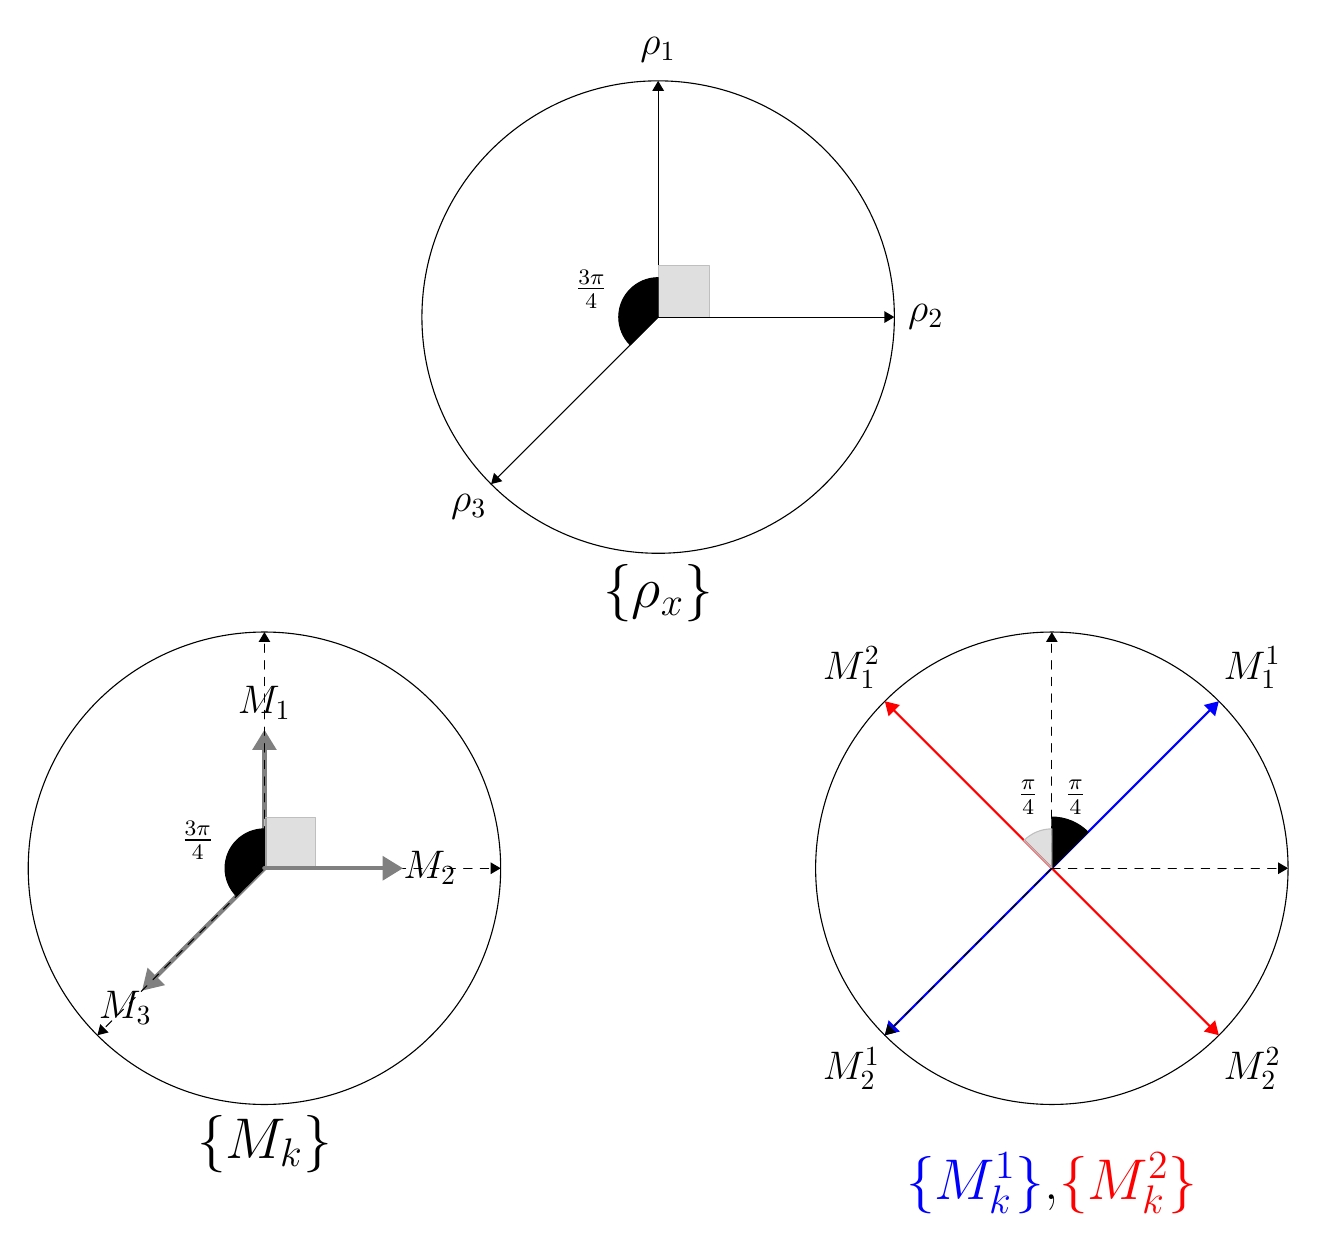
\begin{tikzpicture}[line cap=round, line join=round, >=Triangle]

\begin{scope}[ shift={(0,0)}]
\draw  (0,0) ellipse (3 and 3);


\draw[->]  (0,0) -- (0,3);
\draw (0,3.4) node {\Large $\rho_1$};
\draw [shift={(0,0)},lightgray, fill, fill opacity=0.5] (0,0) rectangle (0.65,0.65);


\begin{scope}[rotate=135]
    \draw[->]  (0,0) -- (0,3);
	\draw (0,3.4) node {\Large $\rho_3$};
	
\draw [shift={(0,0)}, fill] (0,0) -- (90:0.5) arc (90:-45:0.5) -- cycle;
\node at (0.85,0.35) {\large $\frac{3\pi}{4}$};
\end{scope}

\begin{scope}[rotate=-90]    
	\draw[->]  (0,0)  -- (0,3);
	\draw (0,3.4) node {\Large $\rho_2$};
\end{scope}
\node at (0,-3.5) {\huge $\{\rho_x\}$ };
\end{scope}


\begin{scope}[ shift={(-5,-7)}]
\draw  (0,0) ellipse (3 and 3);


\draw[->,ultra thick, gray]  (0,0) -- (0,1.76);
\draw (0,2.1) node {\Large $M_{1}$};
\draw [shift={(0,0)},lightgray, fill, fill opacity=0.5] (0,0) rectangle (0.65,0.65);
\draw[->,dashed]  (0,0) -- (0,3);
\begin{scope}[rotate=135]
   \draw[->,ultra thick,gray]  (0,0) -- (0,2.2);
\draw (0,2.5) node {\Large $M_{3}$};
	\draw[->,dashed]  (0,0) -- (0,3);
\draw [shift={(0,0)}, fill] (0,0) -- (90:0.5) arc (90:-45:0.5) -- cycle;
\node at (0.85,0.35) {\large $\frac{3\pi}{4}$};
\end{scope}

\begin{scope}[rotate=-90]    
\draw[->,dashed]  (0,0) -- (0,3);
	\draw[->,ultra thick,gray]  (0,0) -- (0,1.76);
\draw (0,2.1) node {\Large $M_{2}$};
\end{scope}
\node at (0,-3.5) {\huge $\{M_k\}$ };
\end{scope}



\begin{scope}[ shift={(5,-7)},rotate=-45]
\draw  (0,0) ellipse (3 and 3);


\draw[->,color=blue, thick]  (0,0) -- (0,3);

\draw[->,color=blue, thick]  (0,0) -- (0,-3);
\draw (0,3.6) node {\Large $M^{1}_1$};
\draw (0,-3.6) node {\Large $M^{1}_2$};

 \end{scope}

\begin{scope}[shift={(5,-7)},rotate=45]

    \draw[->,color=red, thick]  (0,0) -- (0,3);
    \draw[->,color=red, thick]  (0,0) -- (0,-3);
	\draw (0,3.6) node {\Large $M^{2}_1$};
	\draw (0,-3.6) node {\Large  $M^{2}_2$};


\end{scope}

\begin{scope}[ shift={(5,-7)}]

\draw[->,dashed]  (0,0) -- (0,3);
\draw [shift={(0,0)}, fill] (0,0) -- (90:0.65) arc (90:45:0.65) -- cycle;
\node at (0.3,0.9) {\large $\frac{\pi}{4}$};
\draw [shift={(0,0)}, lightgray, fill, fill opacity=0.5] (0,0) -- (90:0.5) arc (90:135:0.5) -- cycle;
\node at (-0.3,0.9)  {\large $\frac{\pi}{4}$};
\begin{scope}[rotate=135]
    \draw[->,dashed]  (0,0) -- (0,3);
	
\end{scope}

\begin{scope}[rotate=-90]    
	\draw[->,dashed]  (0,0)  -- (0,3);
	
\end{scope}
\end{scope}


\node at (5,-11) {\huge {\color{blue} $\{M^{1}_k\}$},{\color{red} $\{M^{2}_k\}$}};
\end{tikzpicture}

\end{document}